\documentclass[Xcolor=svgnames,mathserif]{beamer}
\usepackage[utf8]{inputenc}
\usepackage[T1]{fontenc}

\usepackage[english]{babel}
% pour les images
\usepackage{graphicx}
% pour les espaces entre les lignes : 1, 1.5, 2
\usepackage{setspace}
% pour les marges
\usepackage{geometry}
%infos générales du document
\usepackage{amsmath,amsfonts}
% pour les couleurs
\usepackage{color}
% pour mettre des url
\usepackage{url}
% pour les schémas
\usepackage[all]{xy}
% for bold symbols in mathmode
\usepackage{bm}
% biblio exotique
\usepackage{natbib}

\usetheme{metropolis}

% Customisation of the metropolis theme
\definecolor{deeppurple}{HTML}{29293D}
\definecolor{lightpurple}{HTML}{B3B3CC}
\definecolor{medpurple}{HTML}{666699}

\definecolor{deepblue}{HTML}{19194D}
\definecolor{medblue}{HTML}{333399}
\definecolor{lightblue}{HTML}{B3B3E6}


\definecolor{mygreen}{HTML}{3E750A}
\definecolor{mypink}{HTML}{B30047}
%% \definecolor{mypink}{HTML}{CC0052}

\setbeamercolor{normal text}{fg=deeppurple}
\setbeamercolor{frametitle}{bg=deeppurple}
\setbeamercolor{example text}{fg=mypink}
\setbeamercolor{accent text}{fg=myblue}
\setbeamercolor{alerted text}{fg=mypink}
\setbeamercolor{progress bar}{fg=mypink}

\metroset{sectionpage=progressbar, subsectionpage=none, progressbar=frametitle}


\newcommand{\R}{\mathbb{R}}
\newcommand{\beq}{\begin{equation}}
\newcommand{\eeq}{\end{equation}}
\newcommand{\m}[1]{\mathbf{#1}}
\newcommand{\Rlogo}{
\includegraphics[width=0.05\textwidth]{figs/Rlogo-transp}~}
%% \newcommand{\outbreakerlogo}{\raisebox{-0.3mm}{\includegraphics[width=0.25\textwidth]{figs/logo-w300}}~}
%% \newcommand{\outbreakerlogotitle}{\includegraphics[width=.4\textwidth]{figs/logo-w300}~}

% \title[A community for outbreak response tools]{Building a community for the development of outbreak response tools}

\title[R Epidemics Consortium]{
\includegraphics[width=.4\textwidth]{figs/recon-logo.png}}

\subtitle{A graph-based evidence synthesis approach for outbreak detection}

\author[T. Jombart]{Thibaut Jombart}

\institute{Imperial College London\\MRC Centre for Outbreak Analysis and Modelling}
\date{20th September 2017}

% \institute[Imperial College London]{\tiny{MRC Centre for Outbreak Analysis and Modelling \\ Imperial College London}}
% \date[27-06-2014]{~\\3$^e$ rencontres \Rlogo --- Montpellier 27th June 2014}



%% \AtBeginSection[]
%% {
%%  \begin{frame}<beamer>
%%    \frametitle{Outline}
%%    % \tableofcontents[currentsection,currentsubsection]
%%    \tableofcontents[currentsection]
%%  \end{frame}
%% }

% 
% % \addtobeamertemplate{footline}{\hfill\insertframenumber/\inserttotalframenumber\hspace{1em}\vspace{.5em}\null}
% \addtobeamertemplate{footline}{\hfill\vspace{-.35cm}\insertframenumber/\inserttotalframenumber\hspace{1cm}\null}
% 

\usebackgroundtemplate{
  \vspace{-2.5cm}\hspace{-.75cm}
\includegraphics[width=1.3\textwidth]{background.png}
}




\begin{document}





%%%%%%%%%%%%%%%%%%%%%%%%%%%%
%%%%%%%%%%%%%%%%%%%%%%%%%%%%
\begin{frame}[fragile]
  \frametitle{~}
  \vspace{-.3cm}
  %% 
\includegraphics[width=0.2\textwidth]{figs/logoMRC}\hspace*{0.6\textwidth}
\includegraphics[width=0.2\textwidth]{figs/IClogotransp}\\
  %% \vspace{.3cm}
  \titlepage
\end{frame}
%%%%%%%%%%%%%%%%%%%%%%%%%%%%
%%%%%%%%%%%%%%%%%%%%%%%%%%%%






%% %%%%%%%%%%%%%%%%%%%%%%%%%%%%
%% %%%%%%%%%%%%%%%%%%%%%%%%%%%%
%% \begin{frame}{Outline}
%%   \setbeamertemplate{section in toc}[sections numbered]
%%   \tableofcontents[hideallsubsections]
%% \end{frame}
%% %%%%%%%%%%%%%%%%%%%%%%%%%%%%
%% %%%%%%%%%%%%%%%%%%%%%%%%%%%%






%%%%%%%%%%%%%%%%%%%%%%%%%%%%
%%%%%%%%%%%%%%%%%%%%%%%%%%%%
\begin{frame}[fragile]
  \frametitle{Topics of the day}

  \vspace{-1cm}
  \begin{center} 

    \only<1>{
\includegraphics[width=.9\textwidth]{figs/topics1}}\only<2>{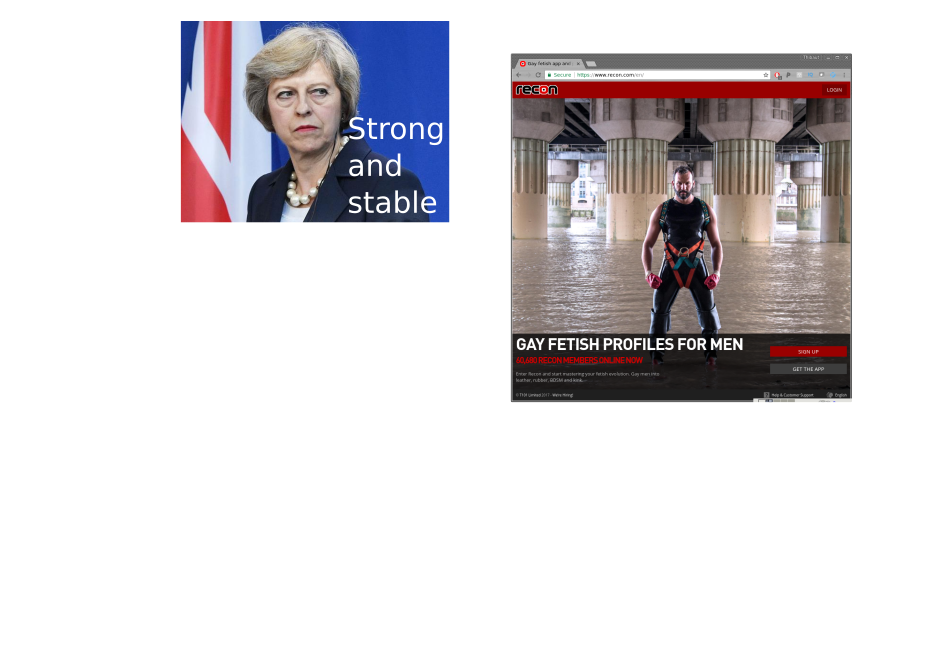
\includegraphics[width=.9\textwidth]{figs/topics2}}\only<3->{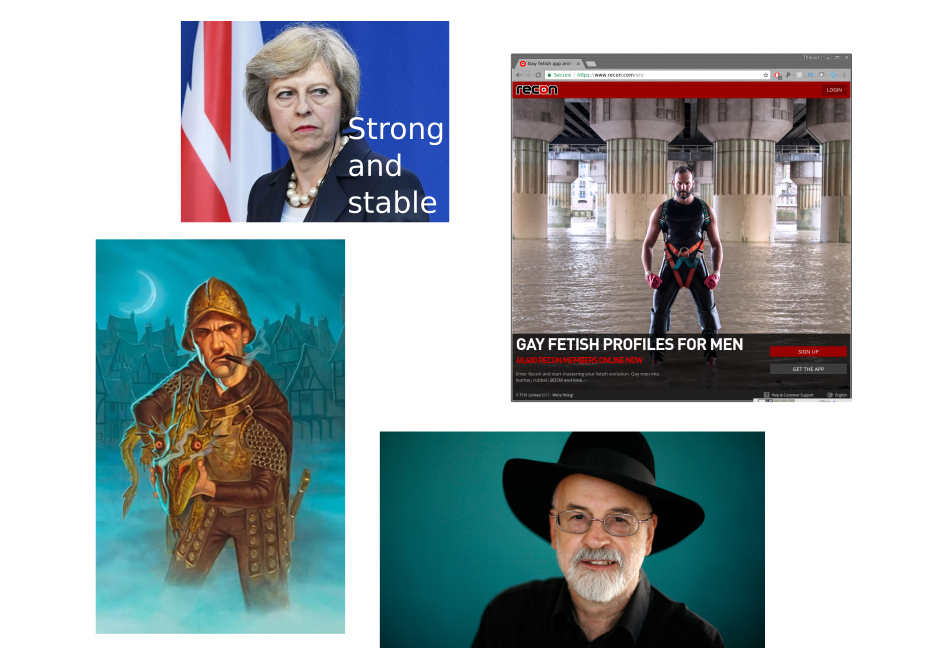
\includegraphics[width=.9\textwidth]{figs/topics3}}

  \end{center}


\end{frame}
%%%%%%%%%%%%%%%%%%%%%%%%%%%%
%%%%%%%%%%%%%%%%%%%%%%%%%%%%







%%%%%%%%%%%%%%%%%%%%%%%%%%%%
%%%%%%%%%%%%%%%%%%%%%%%%%%%%
\section{The R Epidemics Consortium}
%%%%%%%%%%%%%%%%%%%%%%%%%%%%
%%%%%%%%%%%%%%%%%%%%%%%%%%%%




%%%%%%%%%%%%%%%%%%%%%%%%%%%%
%%%%%%%%%%%%%%%%%%%%%%%%%%%%
\begin{frame}[fragile]
  \frametitle{Lessons learnt from the Ebola response}

  \vspace{-1cm}
  \begin{center} 

    \only<1>{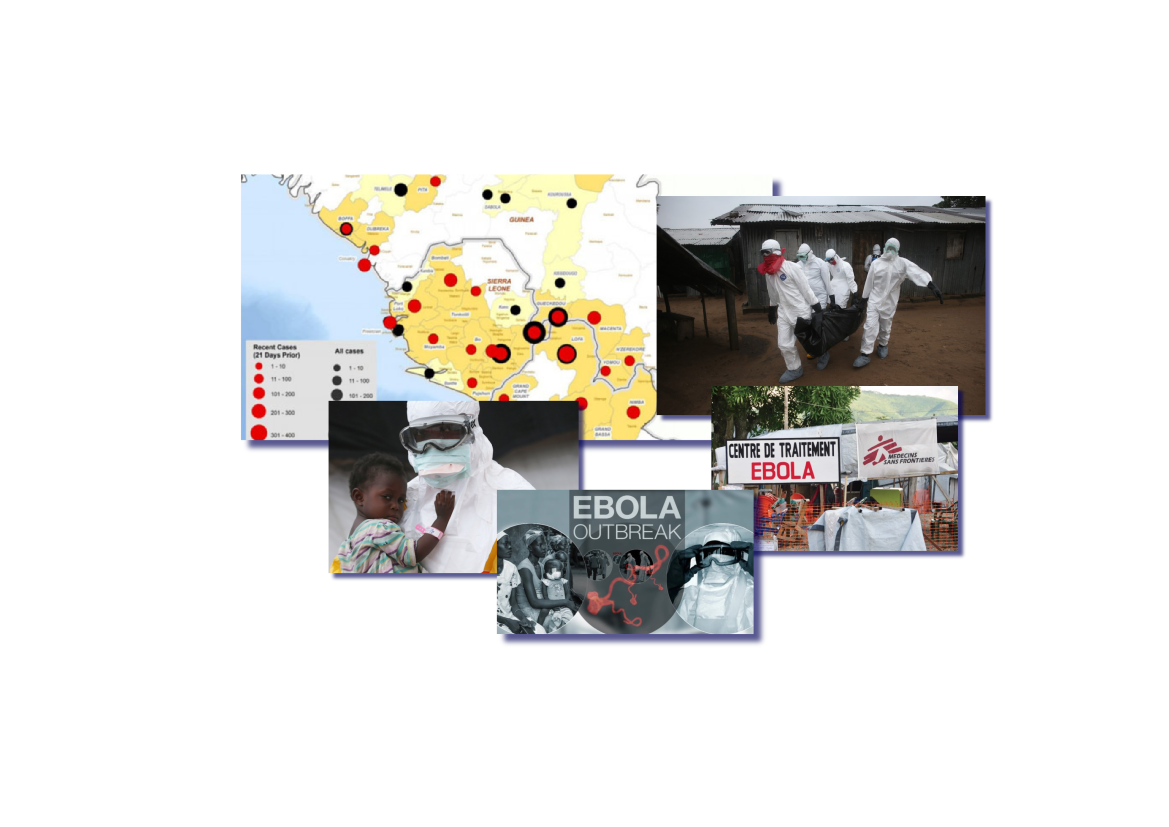
\includegraphics[width=.9\textwidth]{figs/motivation1}}\only<2>{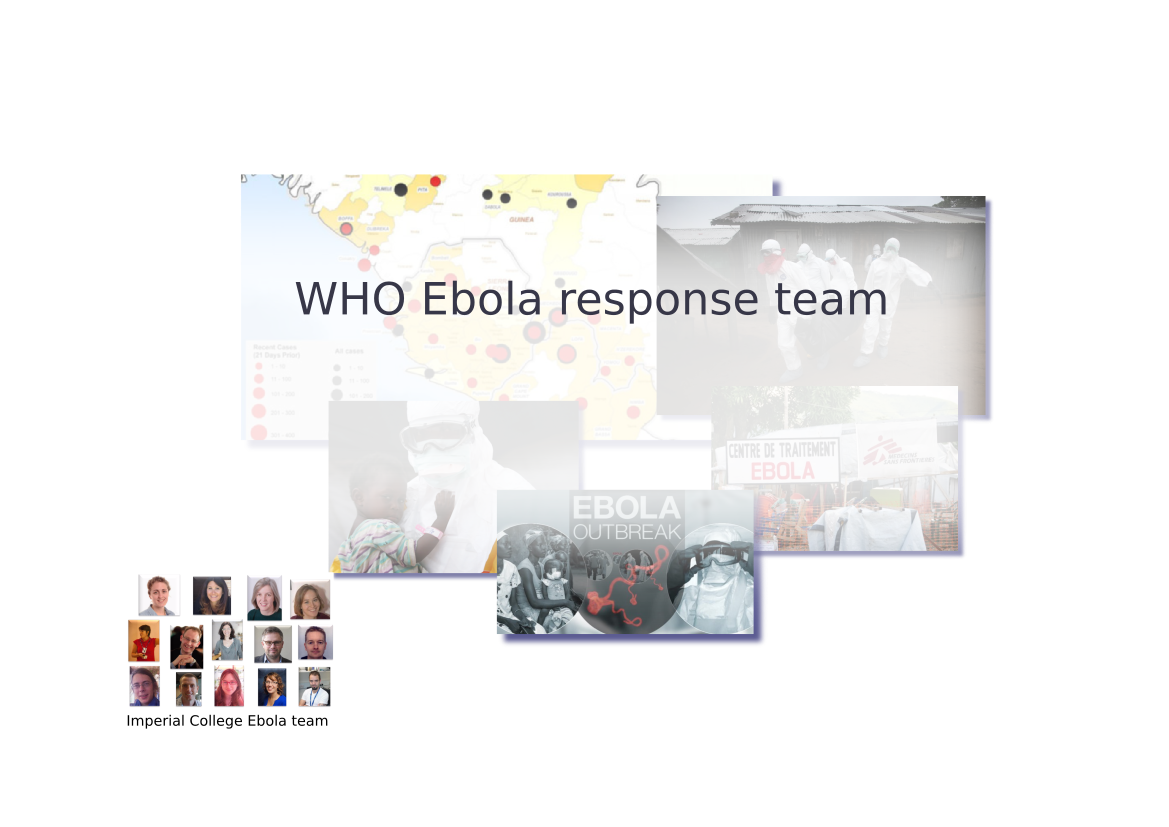
\includegraphics[width=.9\textwidth]{figs/motivation2}}\only<3->{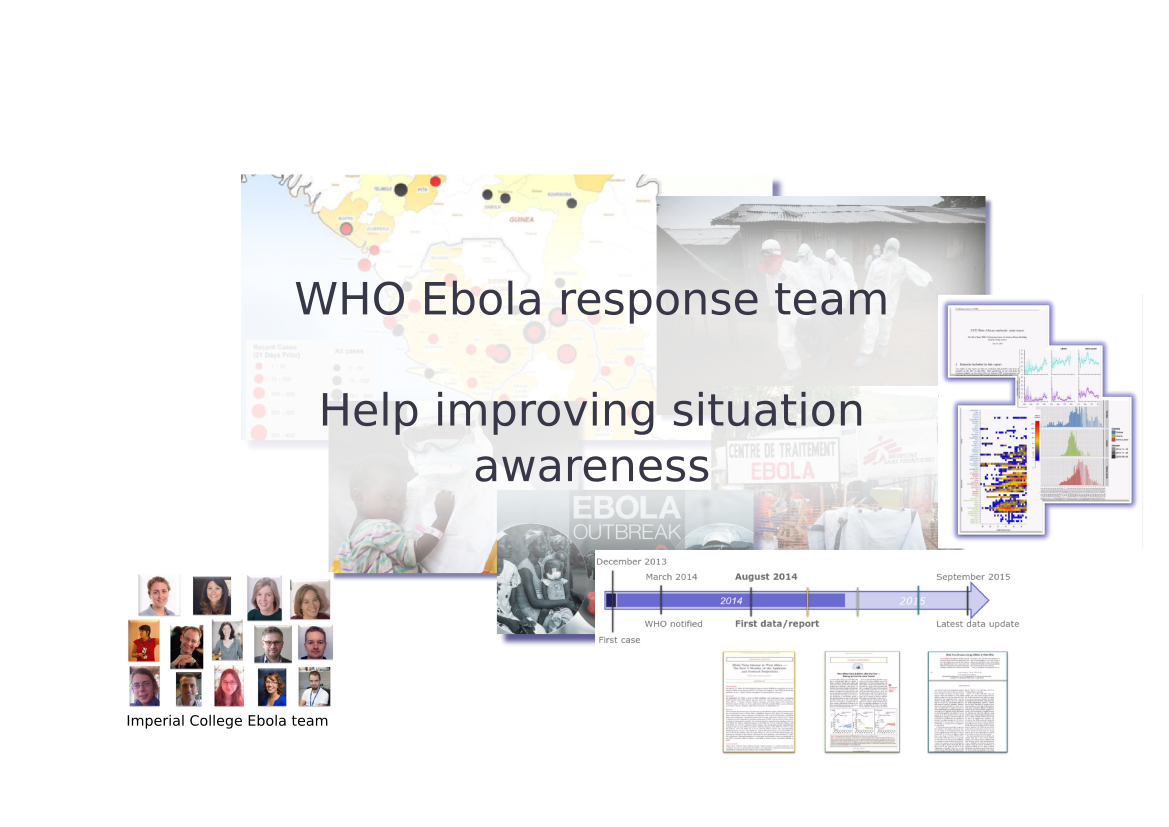
\includegraphics[width=.9\textwidth]{figs/motivation3}}


    \visible<4>{\emph{Most statistical/modelling tools for situation awareness were missing.}}

  \end{center}


\end{frame}
%%%%%%%%%%%%%%%%%%%%%%%%%%%%
%%%%%%%%%%%%%%%%%%%%%%%%%%%%






%%%%%%%%%%%%%%%%%%%%%%%%%%%%
%%%%%%%%%%%%%%%%%%%%%%%%%%%%
\begin{frame}[fragile]
  \frametitle{Who do we need to develop these tools?}

  \vspace{-.5cm}
  \begin{center} 

    \only<1>{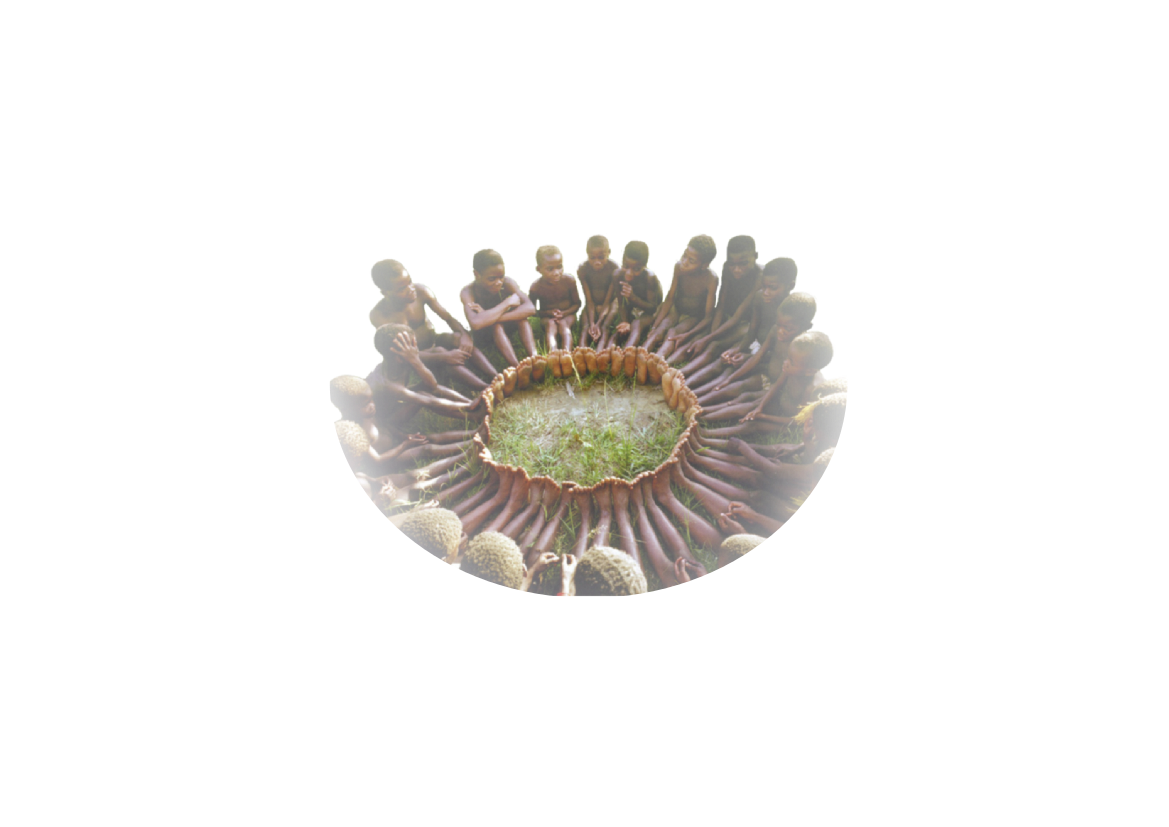
\includegraphics[width=.8\textwidth]{figs/worlds1}}\only<2>{
\includegraphics[width=.8\textwidth]{figs/worlds2}}\only<3>{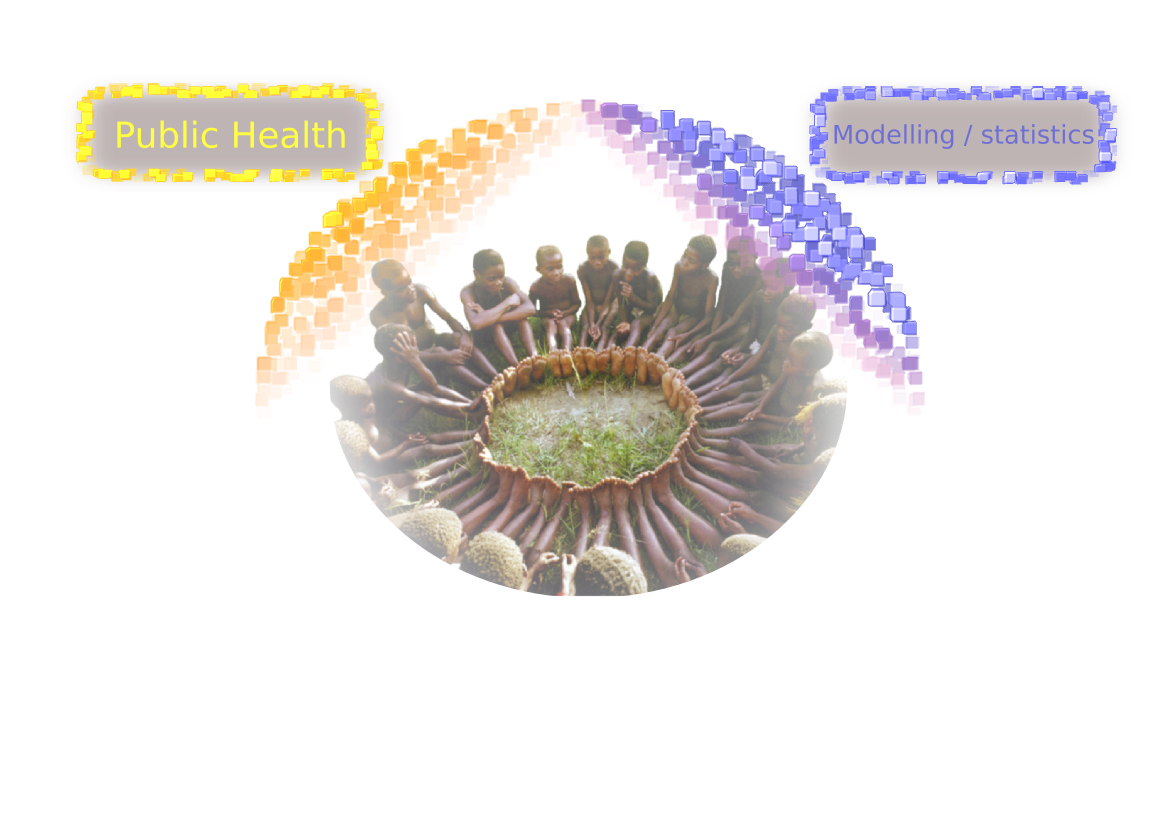
\includegraphics[width=.8\textwidth]{figs/worlds3}}\only<4->{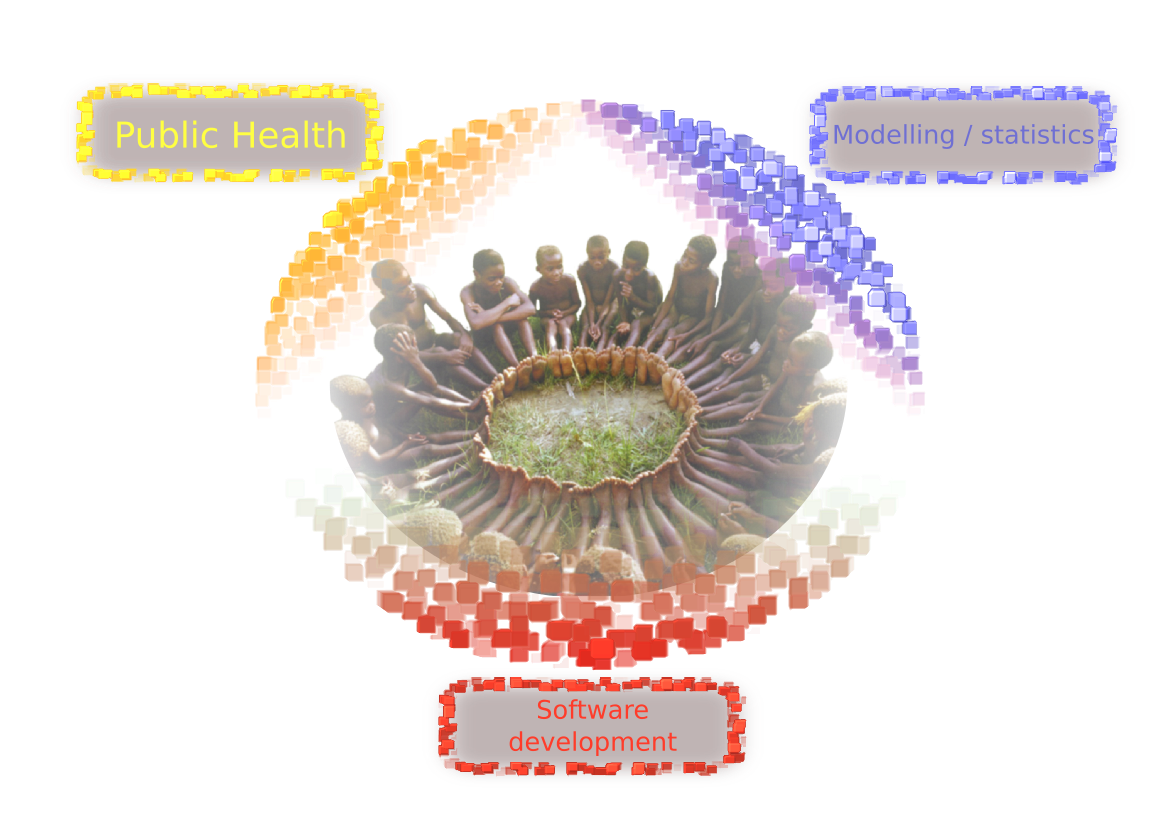
\includegraphics[width=.8\textwidth]{figs/worlds4}}

  \end{center}


\end{frame}
%%%%%%%%%%%%%%%%%%%%%%%%%%%%
%%%%%%%%%%%%%%%%%%%%%%%%%%%%






%%%%%%%%%%%%%%%%%%%%%%%%%%%%
%%%%%%%%%%%%%%%%%%%%%%%%%%%%
\begin{frame}[fragile]
  \frametitle{From a hack to a pack}

  \vspace{-.3cm}
  \begin{center} 
    \only<1>{
\includegraphics[width= \textwidth]{figs/reconbirth1}}\only<2>{
\includegraphics[width= \textwidth]{figs/reconbirth2}}\only<3>{
\includegraphics[width= \textwidth]{figs/reconbirth3}}\only<4->{
\includegraphics[width= \textwidth]{figs/reconbirth4}}
  \end{center}


\end{frame}
%%%%%%%%%%%%%%%%%%%%%%%%%%%%
%%%%%%%%%%%%%%%%%%%%%%%%%%%%






%%%%%%%%%%%%%%%%%%%%%%%%%%%%
%%%%%%%%%%%%%%%%%%%%%%%%%%%%
\begin{frame}[fragile]
  \frametitle{RECON: the \textbf{R} \textbf{E}pidemics \textbf{Con}sortium}
  
  %% \vspace{-.2cm}
  \small A taskforce to build a new generation of outbreak response tools in \Rlogo.

  \vspace{-1cm}
  \begin{center}
    
    \only<1>{
\includegraphics[width=1.1\textwidth]{figs/usnotus1}}\only<2>{
\includegraphics[width=1.1\textwidth]{figs/usnotus2}}\only<3->{
\includegraphics[width=1.1\textwidth]{figs/usnotus3}}

    ~\\
    {\tiny \emph{\url{www.repidemicsconsortium.org}}}
  \end{center}


\end{frame}
%%%%%%%%%%%%%%%%%%%%%%%%%%%%
%%%%%%%%%%%%%%%%%%%%%%%%%%%%






%%%%%%%%%%%%%%%%%%%%%%%%%%%%
%%%%%%%%%%%%%%%%%%%%%%%%%%%%
\begin{frame}[fragile]
  \frametitle{In a nutshell}

  
\includegraphics[width=.5 \textwidth]{figs/recon-logo}
  ~\\
  \emph{\url{www.repidemicsconsortium.org}}

  \begin{itemize}
    
  \item started 6th September 2016 
    %   \pause
    \vspace{.2cm}
  \item $\sim$70 members
    %   \pause
    \vspace{.2cm}
  \item 17 countries, $>$ 40 institutions
    %   \pause
    \vspace{.2cm}
  \item $\sim$ 3 packages released, 20 under development
    %   \pause
    \vspace{.2cm}
  \item public forum, blog, online resources
  \end{itemize}

\end{frame}
%%%%%%%%%%%%%%%%%%%%%%%%%%%%
%%%%%%%%%%%%%%%%%%%%%%%%%%%%





%% %%%%%%%%%%%%%%%%%%%%%%%%%%%%
%% %%%%%%%%%%%%%%%%%%%%%%%%%%%%
%% \begin{frame}[fragile]
%%   \frametitle{The RECON forum}

%% \begin{center}
%% A platform for discussing epidemics analysis in \Rlogo.

%%   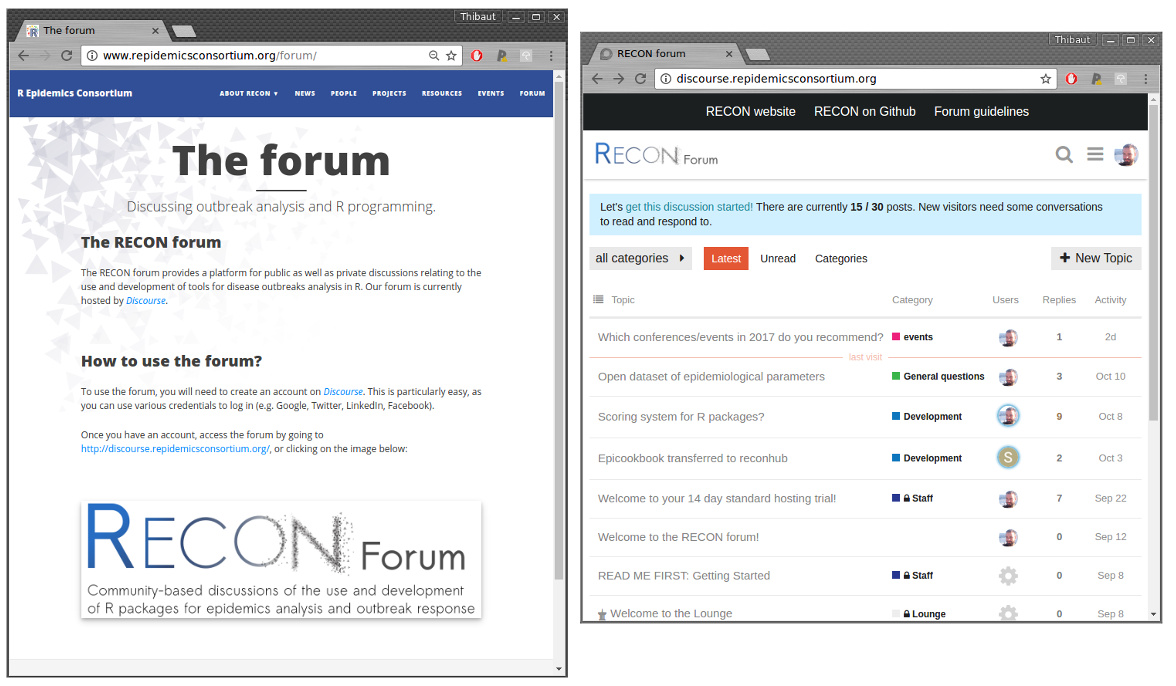
\includegraphics[width=.9\textwidth]{figs/forum}\\
%% \vspace{-.35cm}
%% {\tiny \emph{\url{www.repidemicsconsortium.org/forum}}}
%% \pause
%% ~\\
%% \huge{\alert{Join us!}}

%% \end{center}


%% \end{frame}
%% %%%%%%%%%%%%%%%%%%%%%%%%%%%%
%% %%%%%%%%%%%%%%%%%%%%%%%%%%%%





%%%%%%%%%%%%%%%%%%%%%%%%%%%%
%%%%%%%%%%%%%%%%%%%%%%%%%%%%
\begin{frame}[fragile]
  \frametitle{RECON: what we do}

  \begin{columns}

    \begin{column}{0.2\textwidth}
      \vspace{-3cm}
      \only<1>{
\includegraphics[width=1.2\textwidth]{figs/strongandstable}}
      \only<2->{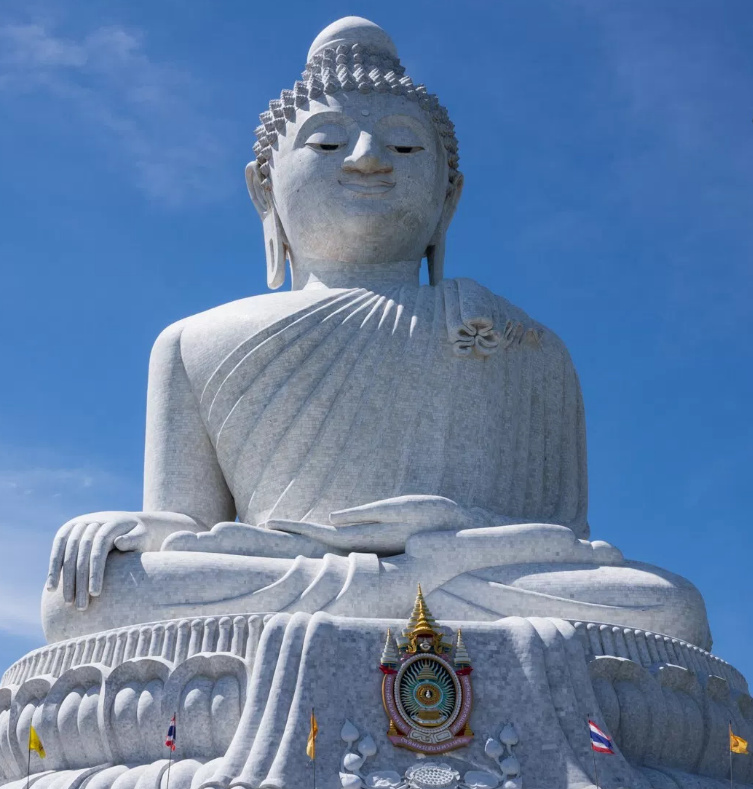
\includegraphics[width=1.2\textwidth]{figs/buddha}\\{\scriptsize $[$nicer\\ 'strong and stable'$]$}}
    \end{column}

    
    \begin{column}{0.8\textwidth}
      \begin{block}{Statistical software development}
        \begin{itemize} 
        \item \alert{efficiency}: useful for improving situation awareness in real time
          %% \pause
        \item \alert{reliability}: outputs can be trusted
          %% \pause
        \item \alert{accessibility}: widely available, easy learning curve
        \end{itemize}
      \end{block}

      \pause
      \pause
      
      \begin{block}{Translation}
        \begin{itemize}
        \item \alert{disseminating knowledge}: free online training material,
          involvement with FETPs, workshops
          %% \pause
        \item \alert{outbreak response}: deployment to the field
        \item \alert{RECON deployer}: portable data analysis environment
        \end{itemize}
      \end{block}


    \end{column}
  \end{columns}

\end{frame}
%%%%%%%%%%%%%%%%%%%%%%%%%%%%
%%%%%%%%%%%%%%%%%%%%%%%%%%%%






%%%%%%%%%%%%%%%%%%%%%%%%%%%%
%%%%%%%%%%%%%%%%%%%%%%%%%%%%
\begin{frame}[fragile]
  \frametitle{RECON: projects}

  \begin{center}
    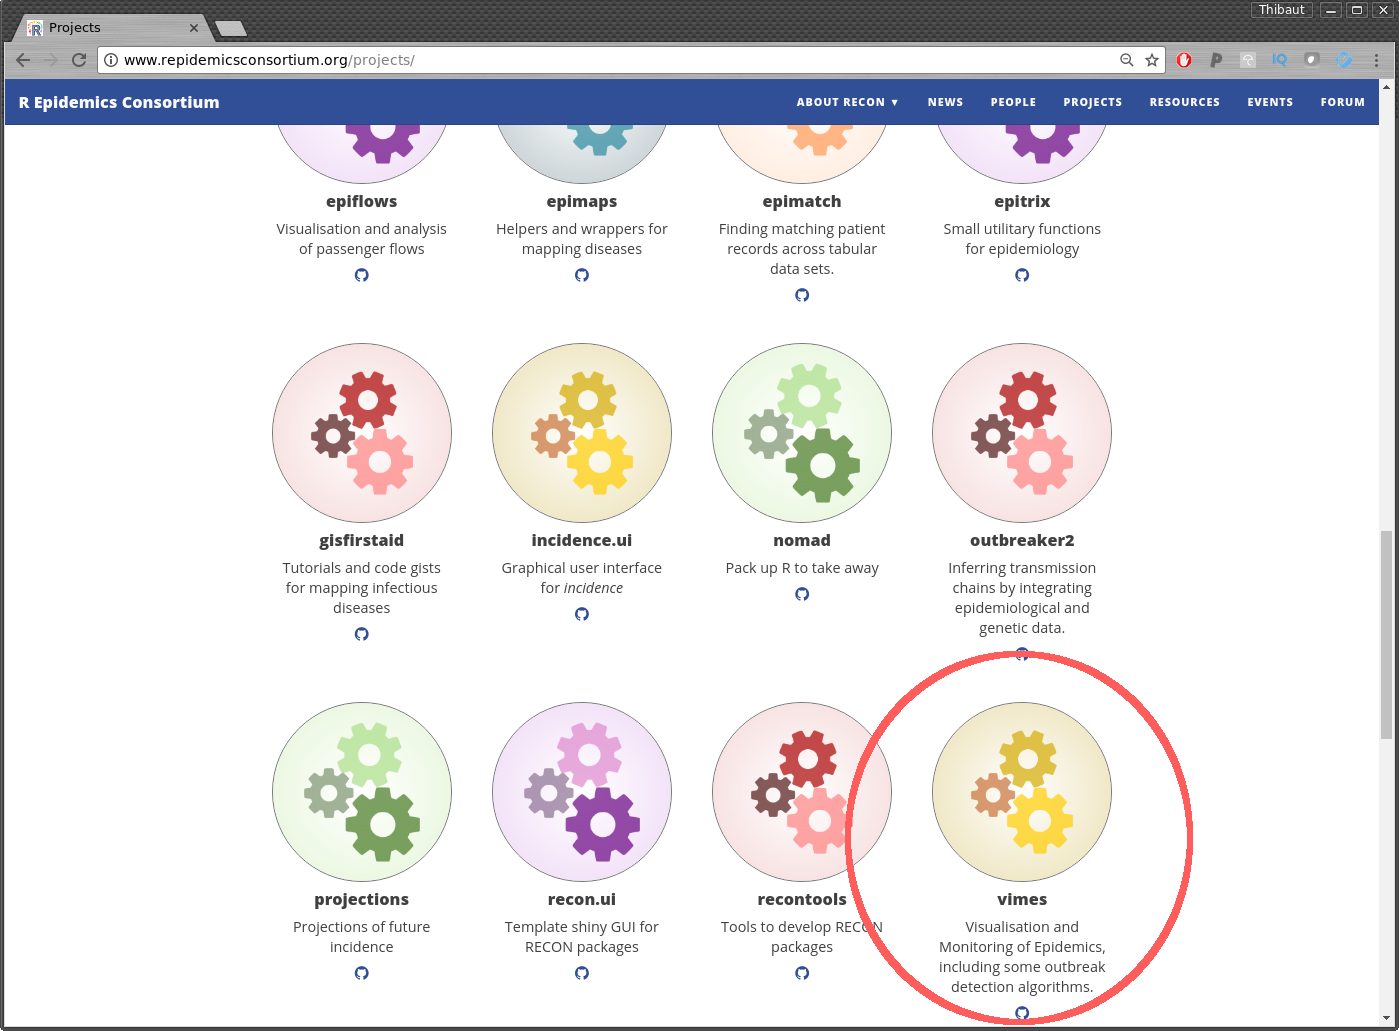
\includegraphics[width=\textwidth]{figs/projectvimes}
  \end{center}

\end{frame}
%%%%%%%%%%%%%%%%%%%%%%%%%%%%
%%%%%%%%%%%%%%%%%%%%%%%%%%%%









%%%%%%%%%%%%%%%%%%%%%%%%%%%%
%%%%%%%%%%%%%%%%%%%%%%%%%%%%
\section{An integrative approach for outbreak detection}
%%%%%%%%%%%%%%%%%%%%%%%%%%%%
%%%%%%%%%%%%%%%%%%%%%%%%%%%%



%%%%%%%%%%%%%%%%%%%%%%%%%%%%
%%%%%%%%%%%%%%%%%%%%%%%%%%%%
\begin{frame}[fragile]
  \frametitle{\alert{VIMES}: \alert{VI}sualisation and \alert{M}onitoring of
    \alert{E}pidemi\alert{S} \footnote[frame]{\tiny well, really, I made that up
      because I was reading 'Snuff' at the time; at least this one is not a
      dodgy website (yet); incidentally, Terry Pratchett was a huge fan of using
      long footnotes, which were often quite entertaining to read; note that it
      does not apply here: if you are still reading this, you probably missed
      what I just said}}
  
  \begin{columns}

    \begin{column}{0.2\textwidth}
      %    \vspace{-4cm}
      \only<1->{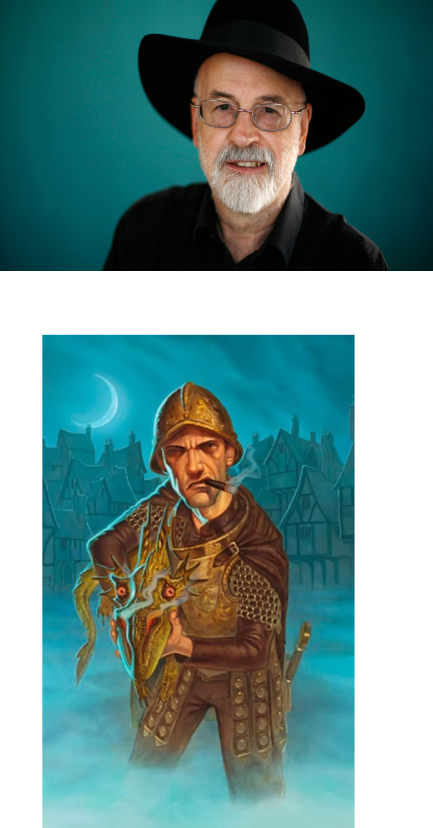
\includegraphics[width=1.2\textwidth]{figs/pratchett}}
    \end{column}
    
    \begin{column}{0.8\textwidth}
      \begin{block}{Aims: develop a new method which..}
        \begin{itemize}
        \item \alert{detects outbreaks} i.e. groups of related cases (on the same transmission chain)
          \pause
        \item \alert{integrates different data}: temporal, spatial, genetic, etc.
          \pause
        \item \alert{works fast, scales well}: so that it can be used for real-time outbreak detection  
        \end{itemize}
      \end{block}


    \end{column}
  \end{columns}


\end{frame}
%%%%%%%%%%%%%%%%%%%%%%%%%%%%
%%%%%%%%%%%%%%%%%%%%%%%%%%%%






%%%%%%%%%%%%%%%%%%%%%%%%%%%%
%%%%%%%%%%%%%%%%%%%%%%%%%%%%
\begin{frame}[fragile]
  \frametitle{A graph-based evidence synthesis approach}
  % \vspace{-.5cm}

  %  \alert{Rationale}:\\data $\rightarrow$ distances $\rightarrow$ graphs $\rightarrow$ clusters
  
  \begin{center}
    
    \only<1>{\resizebox{\textwidth}{!}{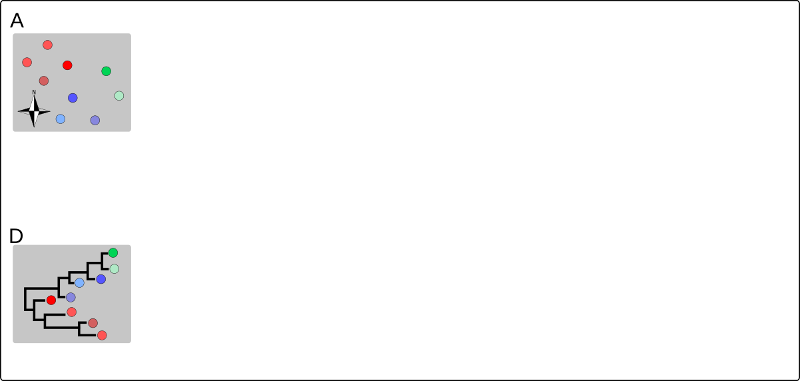
\includegraphics{figs/graphoutbreak1}}}\only<2>{\resizebox{\textwidth}{!}{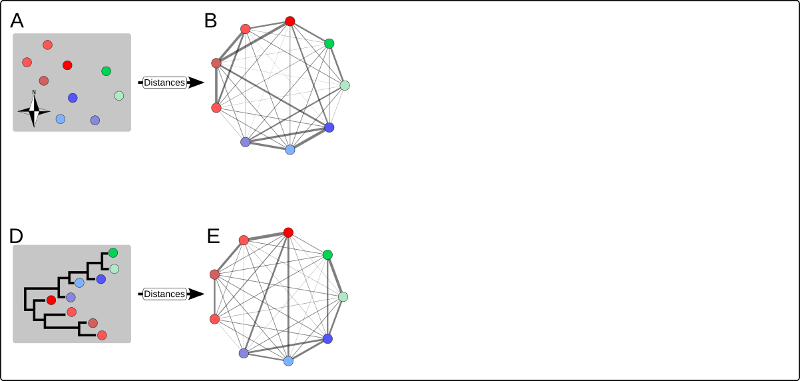
\includegraphics{figs/graphoutbreak2}}}\only<3>{\resizebox{\textwidth}{!}{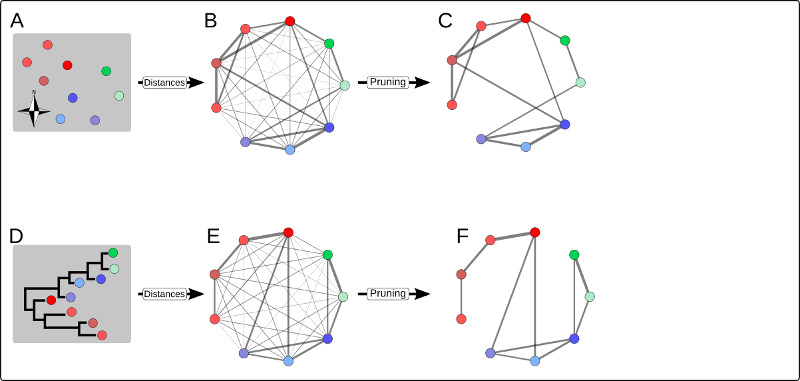
\includegraphics{figs/graphoutbreak3}}}\only<4->{\resizebox{\textwidth}{!}{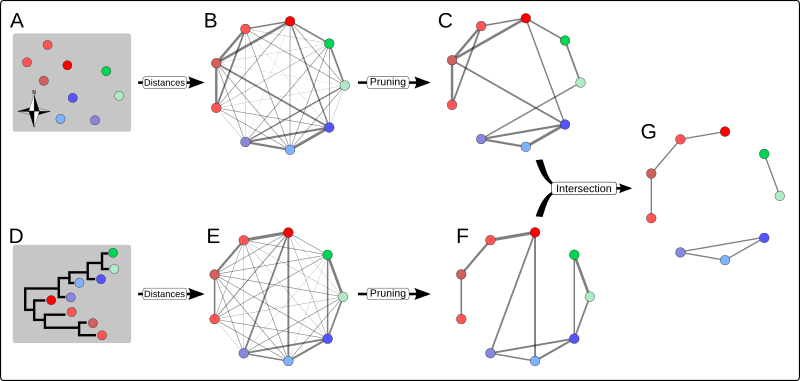
\includegraphics{figs/graphoutbreak4}}}

  \end{center}

\end{frame}
%%%%%%%%%%%%%%%%%%%%%%%%%%%%
%%%%%%%%%%%%%%%%%%%%%%%%%%%%






%%%%%%%%%%%%%%%%%%%%%%%%%%%%
%%%%%%%%%%%%%%%%%%%%%%%%%%%%
\begin{frame}[fragile]
  \frametitle{Pruning graphs: where to cut?}
  % \vspace{-.5cm}

  \only<1>{Assuming a known expected distribution between pairs of cases (e.g. serial interval, spatial kernel, molecular clock), different quantiles can be used:}
  
  \begin{center}
    
    \only<1>{\vspace{.5cm}\resizebox{.65\textwidth}{!}{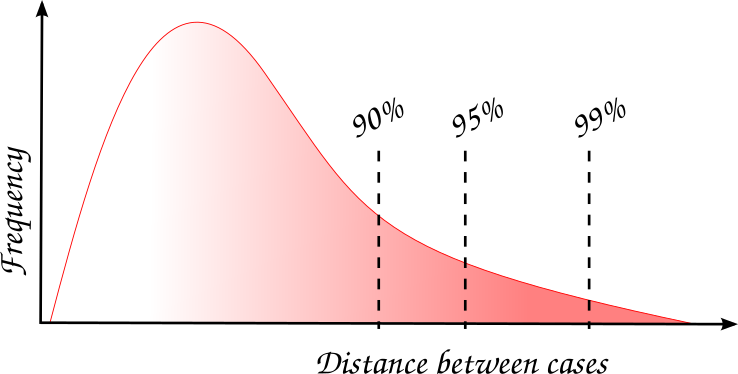
\includegraphics{figs/vimespruning1}}}\only<2->{\vspace{-1cm}}\only<2>{\resizebox{\textwidth}{!}{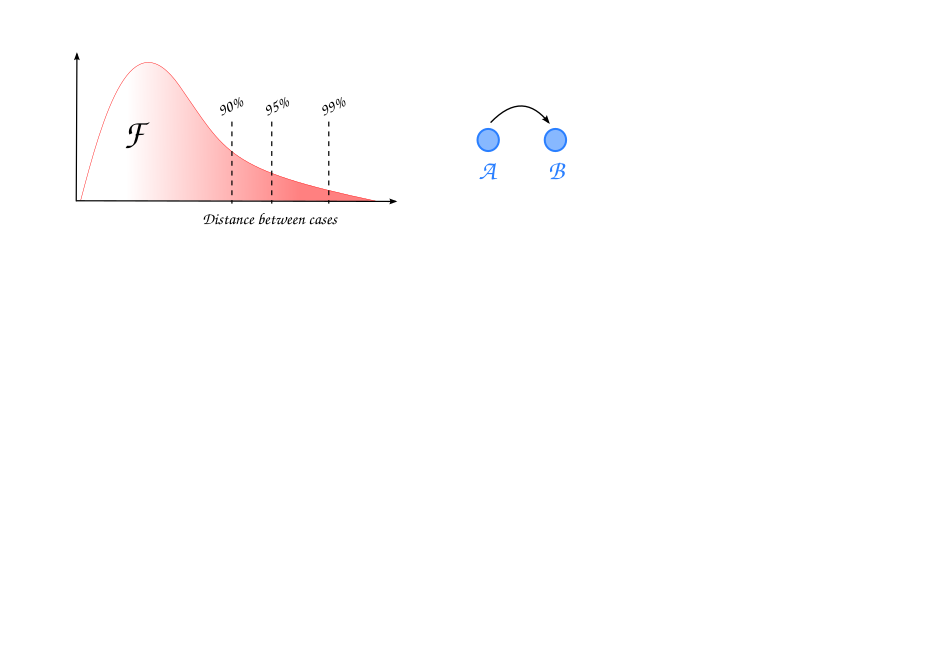
\includegraphics{figs/vimespruning2}}}\only<3>{\resizebox{\textwidth}{!}{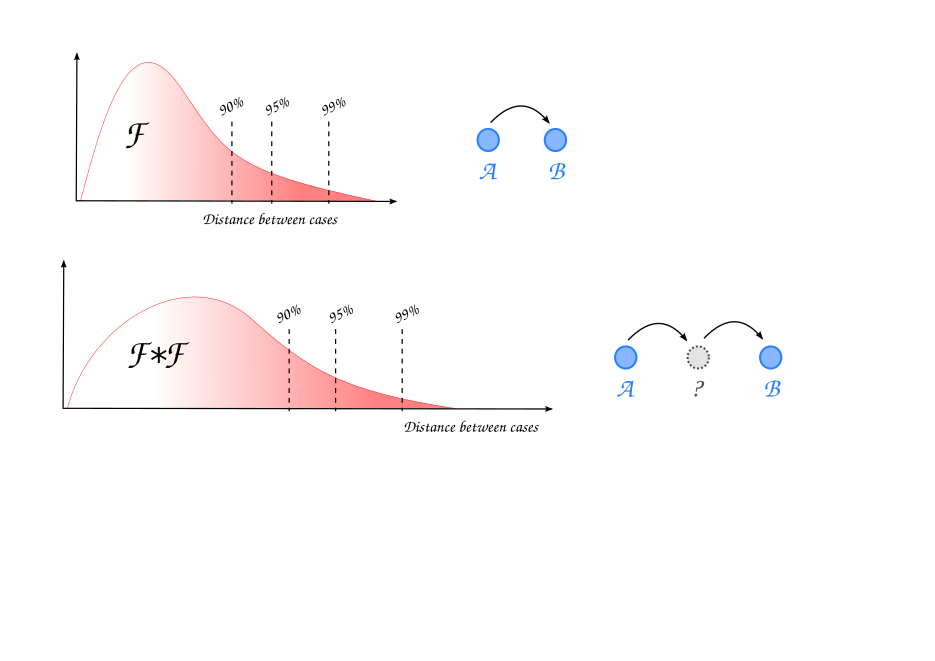
\includegraphics{figs/vimespruning3}}}\only<4>{\resizebox{\textwidth}{!}{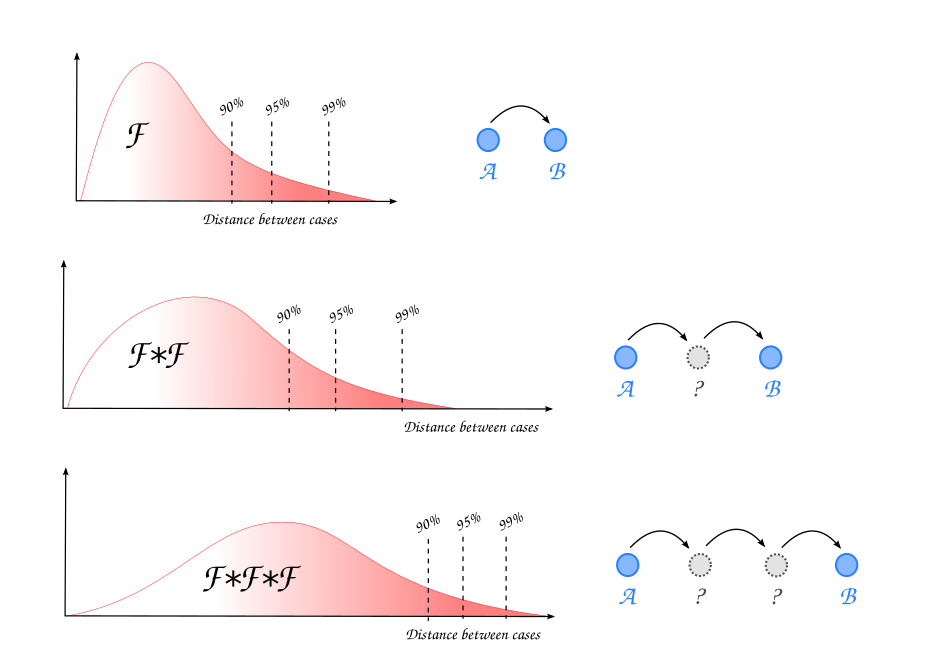
\includegraphics{figs/vimespruning4}}}\only<5>{\resizebox{\textwidth}{!}{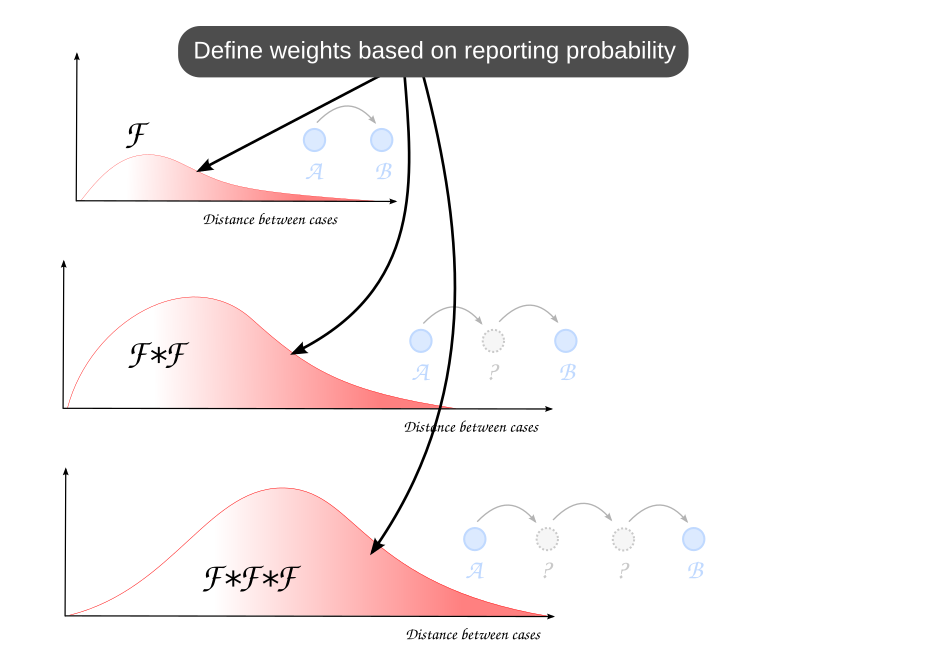
\includegraphics{figs/vimespruning5}}}\only<6->{\resizebox{\textwidth}{!}{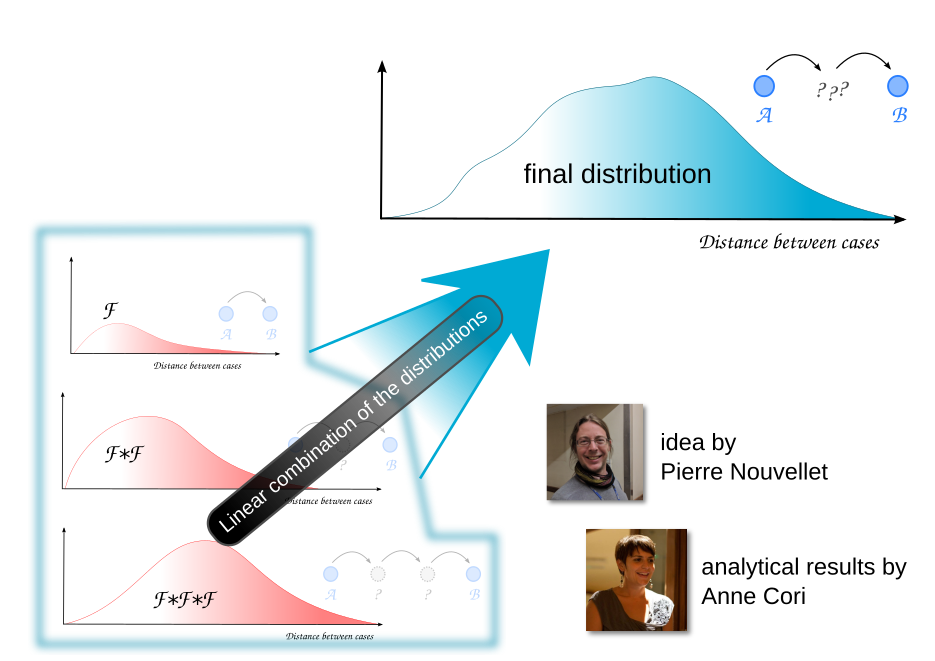
\includegraphics{figs/vimespruning6}}}

  \end{center}

\end{frame}
%%%%%%%%%%%%%%%%%%%%%%%%%%%%
%%%%%%%%%%%%%%%%%%%%%%%%%%%%






%%%%%%%%%%%%%%%%%%%%%%%%%%%%
%%%%%%%%%%%%%%%%%%%%%%%%%%%%
\begin{frame}[fragile]
  \frametitle{Application: dog rabies epidemics, Central African Republic}
  %  \vspace{-.5cm}

  
  \begin{center}
    \resizebox{0.95\textwidth}{!}{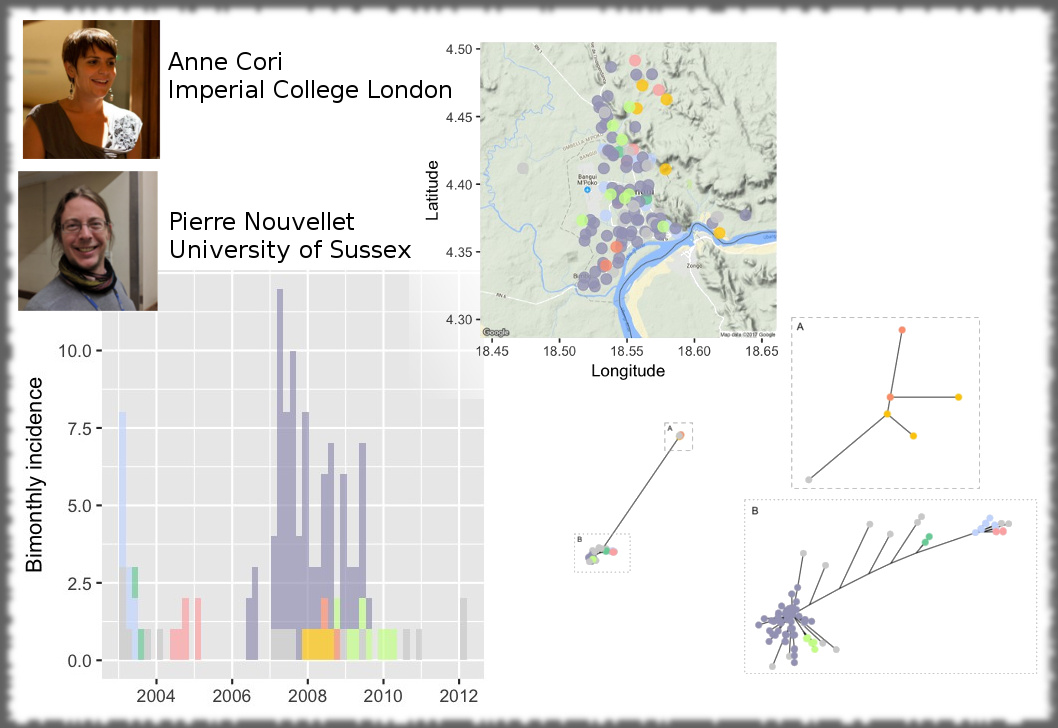
\includegraphics{figs/rabiesdata}}
  \end{center}


\end{frame}
%%%%%%%%%%%%%%%%%%%%%%%%%%%%
%%%%%%%%%%%%%%%%%%%%%%%%%%%%






%%%%%%%%%%%%%%%%%%%%%%%%%%%%
%%%%%%%%%%%%%%%%%%%%%%%%%%%%
\begin{frame}[fragile]
  \frametitle{Distributions of distances between cases}
  %  \vspace{-.5cm}

  
  \begin{center}
    \resizebox{0.95\textwidth}{!}{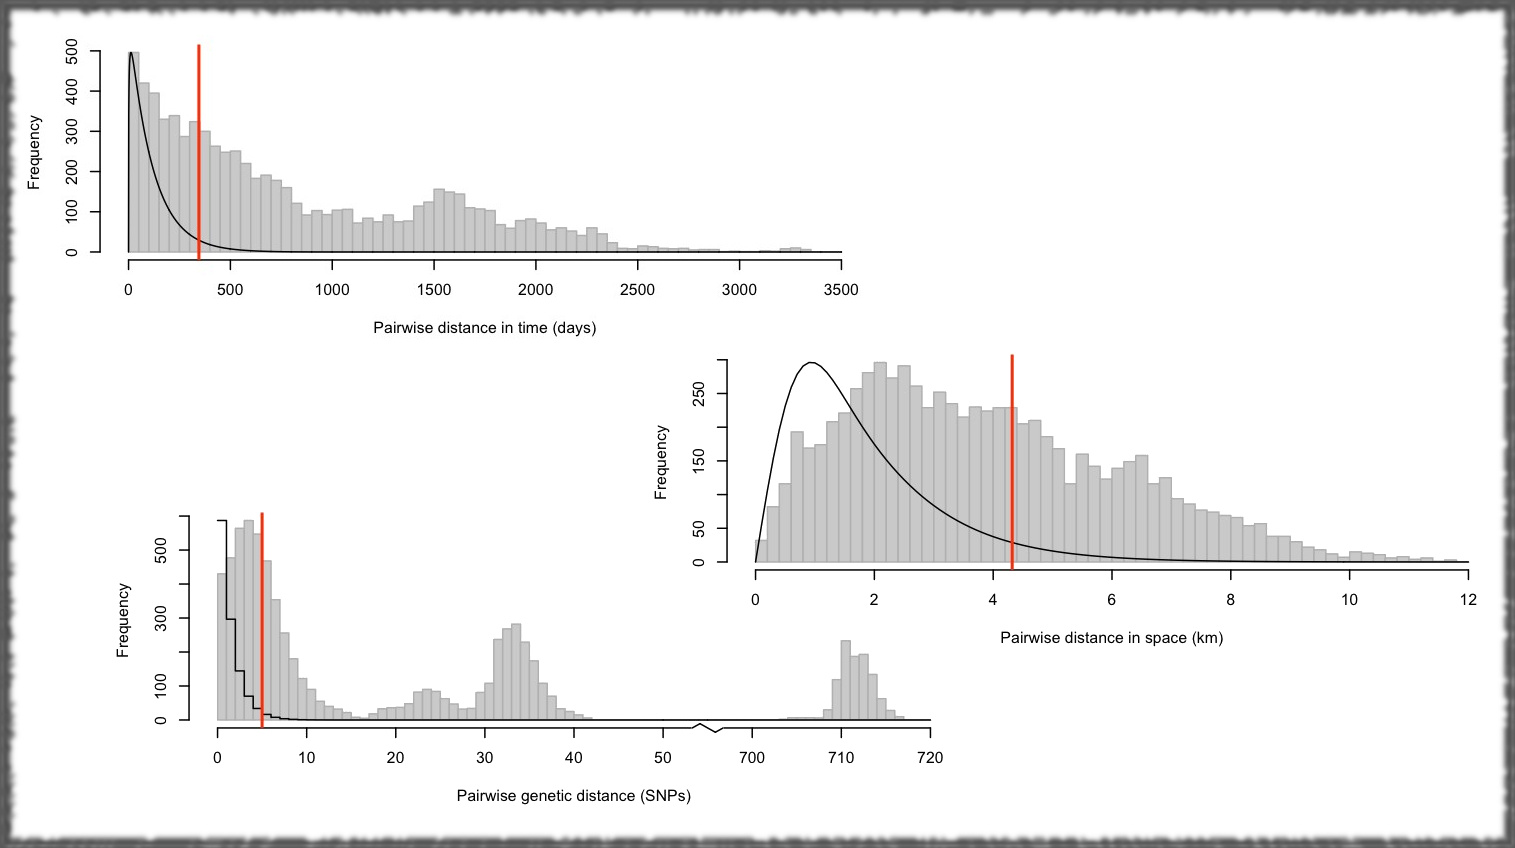
\includegraphics{figs/rabiesdistances}}
    ~\\
              {\footnotesize $[$material by Anne Cori$]$}
  \end{center}


\end{frame}
%%%%%%%%%%%%%%%%%%%%%%%%%%%%
%%%%%%%%%%%%%%%%%%%%%%%%%%%%






%%%%%%%%%%%%%%%%%%%%%%%%%%%%
%%%%%%%%%%%%%%%%%%%%%%%%%%%%
\begin{frame}[fragile]
  \frametitle{Results}
%  \vspace{-.5cm}

  
  \begin{center}
    \only<1>{\resizebox{0.95\textwidth}{!}{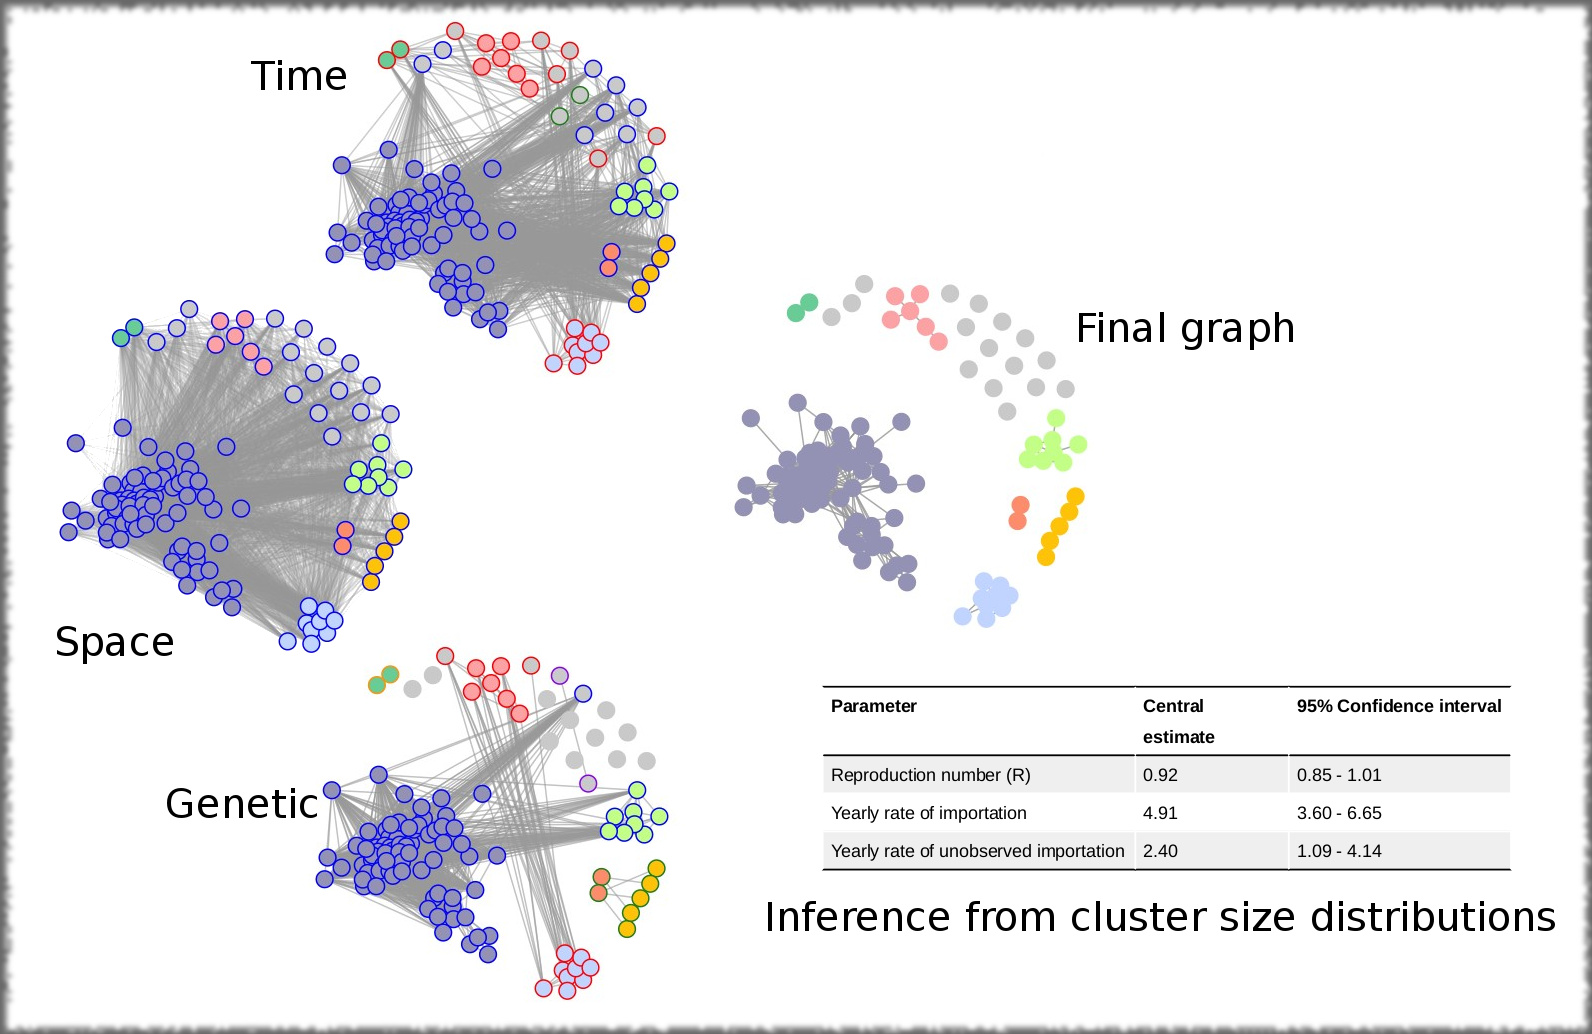
\includegraphics{figs/rabiesresults}}{\\\footnotesize $[$material by Anne Cori and Pierre Nouvellet$]$}}
  \end{center}

  \only<2>{\vspace{-1cm}\resizebox{0.7\textwidth}{!}{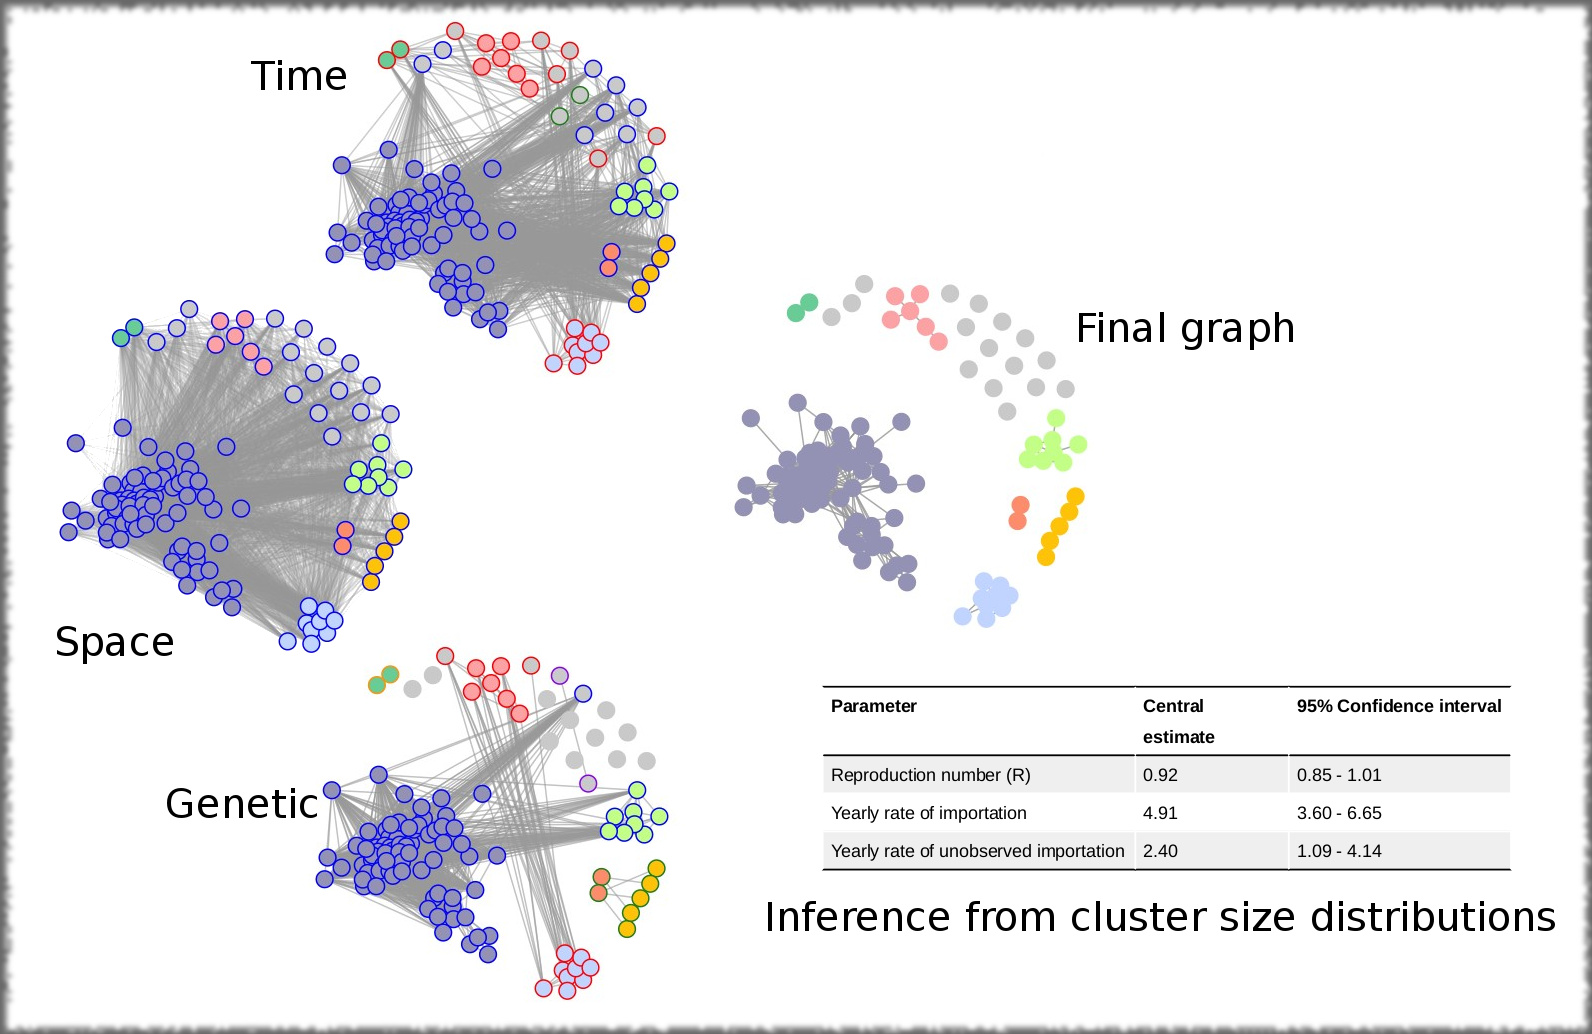
\includegraphics{figs/rabiesresults}}}

  \pause
  \begin{itemize}
  \item one large outbreak, low $R_0$, $\sim 5-10$ introductions / year
  \item same results as more complex approaches (BEAST, epi model + partical filtering)
  \item much faster (<1s $vs$ $~1$ week)
  \end{itemize}

\end{frame}
%%%%%%%%%%%%%%%%%%%%%%%%%%%%
%%%%%%%%%%%%%%%%%%%%%%%%%%%%






%%%%%%%%%%%%%%%%%%%%%%%%%%%%
%%%%%%%%%%%%%%%%%%%%%%%%%%%%
\begin{frame}[fragile]
  \frametitle{Perspectives}
  %  \vspace{-.5cm}

  \begin{itemize}
  \item \alert{flexible} approach for detecting outbreaks using different data types
    \pause
    \vspace{.25cm}
  \item \alert{threshold}: unsatisfying, but sensitivity study easy
    \pause
    \vspace{.25cm}
  \item \alert{fast and scalable}: possible integration in routine surveillance
    \pause
    \vspace{.25cm}
  \item can serve as \alert{basis to other methods} for integrating different data sources
  \end{itemize}

\end{frame}
%%%%%%%%%%%%%%%%%%%%%%%%%%%%
%%%%%%%%%%%%%%%%%%%%%%%%%%%%






%%%%%%%%%%%%%%%%%%%%%%%%%%%%
%%%%%%%%%%%%%%%%%%%%%%%%%%%%
\begin{frame}[fragile]
  \frametitle{Thanks}

  \small
  %% \begin{block}{Thanks to:}
  \begin{itemize}
  \item \alert{Conference organisers}
  \item \alert{Colleagues:} \textbf{Anne Cori}, \textbf{Pierre Nouvellet}, Tini Garske, Hervé Bourhy, Emmanuel Nakouné
  \item \alert{Groups:} WHO Ebola Response Team, Hackout 1/2/3, RECON members, GOARN
  \item \alert{funding:} HPRU-NIHR, MRC
  \end{itemize}
  %% \end{block}

  
  \begin{center}

    \begin{columns}
      \begin{column}{0.5\textwidth}
        \centering
        
\includegraphics[width=.75\textwidth]{figs/recon-logo}
        
        {\footnotesize \emph{\url{www.repidemicsconsortium.org}}}
      \end{column}
      
      \begin{column}{0.5\textwidth}
        \centering
        ~\\~\\~\\
            {\huge \alert{\emph{vimes}}}\\
        {\footnotesize \emph{\url{www.repidemicsconsortium.org/vimes}}}
      \end{column}
    \end{columns}
    \vspace{.3cm}
    {\huge \textbf{Questions?}}
    
  \end{center}

  
\end{frame}
%%%%%%%%%%%%%%%%%%%%%%%%%%%%
%%%%%%%%%%%%%%%%%%%%%%%%%%%%













\end{document}
